\documentclass[12pt]{article}
\usepackage[a4paper,margin=1.25cm]{geometry}
\usepackage{amsmath,amssymb,mathtools}
\usepackage{graphicx}
\usepackage{booktabs}
\usepackage{tabularx}
\usepackage{tikz}
\usepackage[T1]{fontenc}
\usepackage[utf8]{inputenc}
\usepackage[english]{babel}

\setlength{\parindent}{0pt}
\setlength{\parskip}{0.45em}
\setlength{\abovedisplayskip}{5pt plus 1pt minus 1pt}
\setlength{\belowdisplayskip}{5pt plus 1pt minus 1pt}
\setlength{\abovedisplayshortskip}{3pt plus 1pt minus 1pt}
\setlength{\belowdisplayshortskip}{3pt plus 1pt minus 1pt}

\newcommand{\dd}{\,\mathrm{d}}
\newcommand{\ii}{\mathrm{i}}
\newcommand{\e}{\mathrm{e}}
\newcommand{\Log}{\operatorname{Log}}
\newcommand{\Arg}{\operatorname{Arg}}
\newcommand{\D}{\mathbb D}
\newcommand{\Rp}{\operatorname{Re}}
\newcommand{\Ip}{\operatorname{Im}}

\begin{document}

\begin{center}
{\Large\bfseries An integral governed by a strip}\\[0.35em]
{\large the circle mean becomes the density \(\mathrm{d}t/\cosh t\)}
\end{center}

\[
\boxed{\displaystyle
\int_0^\infty
\frac{\sinh x}{x\cosh(x/a)}\dd x
=\log\cot\frac{\pi(1-a)}4,
\qquad 0<a<1.}
\]

\textbf{Overview.}
The \(\cosh\) in the denominator is not an accident of the integrand: it
is the harmonic measure of the boundary of a horizontal strip, pushed
forward from the uniform measure of a circle. The map
\[
\Phi(\zeta)=\Log\frac{1+\zeta}{1-\zeta}
\]
carries the unit disk onto the strip \(|\Ip w|<\pi/2\), and carries the
uniform measure \(\dd\theta\) on the unit circle onto
\(\dd t/\cosh t\) on the two boundary lines. The mean-value property for
holomorphic functions therefore reads, in strip coordinates,
\[
F(0)=\frac1{2\pi}\int_{-\infty}^{\infty}
\frac{F(t+\tfrac{\pi\ii}{2})+F(t-\tfrac{\pi\ii}{2})}{\cosh t}\dd t,
\]
and every integral in this note is one choice of \(F\). Taking
\(F(w)=\e^{sw}\) gives \(\int\e^{st}\operatorname{sech}t\dd t=\pi\sec\frac{\pi s}{2}\);
integrating that in the parameter gives the stated \(\log\cot\).

\section*{0. The range of the parameter}

The problem as posed does not specify which \(a\) are allowed, and the
answer only makes sense for some. At the origin there is no difficulty:
\[
\frac{\sinh x}{x\cosh(x/a)}\longrightarrow1,\qquad x\to0.
\]
At infinity, for \(a>0\),
\[
\frac{\sinh x}{x\cosh(x/a)}
\sim
\frac{\e^{(1-1/a)x}}{x},
\]
which is integrable exactly when \(1-\frac1a<0\). Hence the working range
is
\[
\boxed{0<a<1,}
\]
and note that the right-hand side \(\log\cot\frac{\pi(1-a)}4\) is then
finite and positive, blowing up as \(a\to1^-\) precisely where the
integral diverges.

It is cleaner to prove a two-parameter statement and specialise.

\textbf{Theorem.} For real \(\alpha,\beta\) with \(\beta>0\) and
\(|\alpha|<\beta\),
\[
\boxed{\displaystyle
G(\alpha,\beta)=
\int_0^\infty
\frac{\sinh(\alpha x)}{x\cosh(\beta x)}\dd x
=\log\cot\frac{\pi(\beta-\alpha)}{4\beta}.}
\tag{$\ast$}
\]
The integral of the problem is \(G(1,1/a)\).

\section*{1. The disk becomes a strip}

Let \(\Log z=\log|z|+\ii\Arg z\) with \(-\pi<\Arg z<\pi\), and set
\[
\Phi(\zeta)=\Log\frac{1+\zeta}{1-\zeta},\qquad \zeta\in\D=\{|\zeta|<1\}.
\]
For \(|\zeta|<1\) the M\"obius image \(\frac{1+\zeta}{1-\zeta}\) lies in
the right half-plane \(\Rp z>0\): indeed
\[
\Rp\frac{1+\zeta}{1-\zeta}
=\frac{1-|\zeta|^2}{|1-\zeta|^2}>0 .
\]
So the principal branch is single-valued on \(\D\), and since \(\Log\)
maps the right half-plane onto \(\{|\Ip w|<\pi/2\}\),
\[
\Phi:\D\xrightarrow{\ \sim\ }S=\Bigl\{w:\ |\Ip w|<\frac\pi2\Bigr\},
\qquad \Phi(0)=0.
\tag{1}
\]

\begin{center}
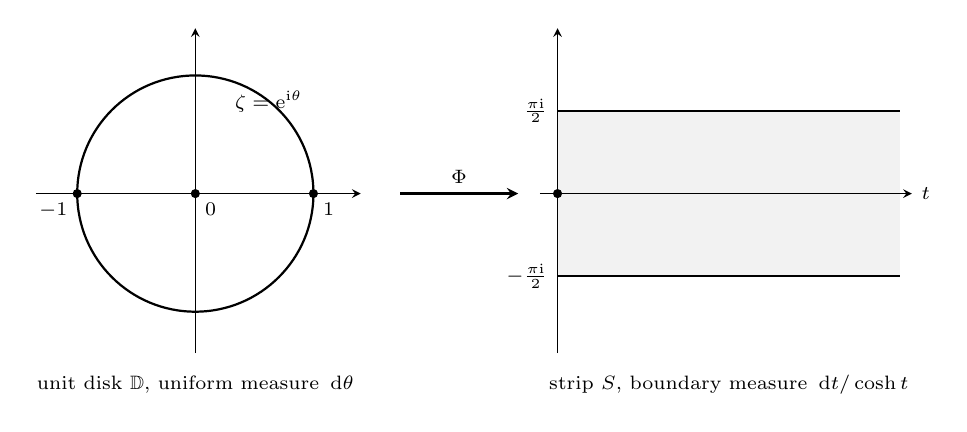
\begin{tikzpicture}[>=stealth]
\begin{scope}[scale=1.5]
  \draw[thick] (0,0) circle (1);
  \draw[->] (-1.35,0)--(1.4,0);
  \draw[->] (0,-1.35)--(0,1.4);
  \fill (0,0) circle (1.1pt) node[below right] {\scriptsize \(0\)};
  \fill (1,0) circle (1.1pt) node[below right] {\scriptsize \(1\)};
  \fill (-1,0) circle (1.1pt) node[below left] {\scriptsize \(-1\)};
  \node at (0.62,0.78) {\scriptsize \(\zeta=\e^{\ii\theta}\)};
  \node at (0,-1.62) {\scriptsize unit disk \(\D\), uniform measure \(\dd\theta\)};
\end{scope}
\draw[->,thick] (2.6,0)--(4.1,0) node[midway,above] {\scriptsize \(\Phi\)};
\begin{scope}[shift={(4.6,0)},scale=1.5]
  \fill[black!5] (0,-0.7) rectangle (2.9,0.7);
  \draw[thick] (0,0.7)--(2.9,0.7);
  \draw[thick] (0,-0.7)--(2.9,-0.7);
  \draw[->] (0,-1.35)--(0,1.4);
  \draw[->] (-0.15,0)--(3.0,0) node[right] {\scriptsize \(t\)};
  \node[left] at (0,0.7) {\scriptsize \(\tfrac{\pi\ii}{2}\)};
  \node[left] at (0,-0.7) {\scriptsize \(-\tfrac{\pi\ii}{2}\)};
  \fill (0,0) circle (1.1pt);
  \node at (1.45,-1.62) {\scriptsize strip \(S\), boundary measure \(\dd t/\cosh t\)};
\end{scope}
\end{tikzpicture}
\end{center}

\section*{2. The boundary measure is \(\mathrm{d}t/\cosh t\)}

Put \(\zeta=\e^{\ii\theta}\). Factoring out the half-angle,
\[
1+\e^{\ii\theta}=2\e^{\ii\theta/2}\cos\frac\theta2,
\qquad
1-\e^{\ii\theta}=-2\ii\,\e^{\ii\theta/2}\sin\frac\theta2,
\]
so
\[
\frac{1+\e^{\ii\theta}}{1-\e^{\ii\theta}}
=\ii\cot\frac{\theta}{2}.
\tag{2}
\]
For \(0<\theta<\pi\) we have \(\cot\frac\theta2>0\), so (2) is a positive
multiple of \(\ii\) and
\[
w=\Phi(\e^{\ii\theta})=t+\frac{\pi\ii}{2},
\qquad
t=\log\cot\frac\theta2 .
\tag{3}
\]
For \(\pi<\theta<2\pi\) the cotangent is negative and the same
computation gives \(w=t-\frac{\pi\ii}{2}\) with
\(t=\log\bigl|\cot\frac\theta2\bigr|\). The upper semicircle covers the
upper boundary line, the lower semicircle the lower one; each covers it
exactly once, since \(\theta\mapsto\log\cot\frac\theta2\) is a decreasing
bijection \((0,\pi)\to(+\infty,-\infty)\).

Now differentiate (3):
\[
\frac{\dd t}{\dd\theta}
=\frac{1}{\cot\frac\theta2}\cdot\Bigl(-\tfrac12\csc^2\tfrac\theta2\Bigr)
=-\frac1{2\sin\frac\theta2\cos\frac\theta2}
=-\frac1{\sin\theta}.
\tag{4}
\]
Next, \(\sin\theta\) can be expressed in \(t\). From \(\cot\frac\theta2=\e^{t}\), i.e. \(\tan\frac\theta2=\e^{-t}\),
\[
\sin\theta
=\frac{2\tan\frac\theta2}{1+\tan^2\frac\theta2}
=\frac{2\e^{-t}}{1+\e^{-2t}}
=\frac{1}{\cosh t}.
\tag{5}
\]
Combining (4) and (5),
\[
\boxed{\displaystyle |\dd\theta|=\frac{\dd t}{\cosh t}.}
\tag{6}
\]
On the lower semicircle the sign of \(\sin\theta\) flips but so does the
orientation, and the same positive density results. This is the origin of
the hyperbolic cosine: it is the Jacobian of the uniformising map,
nothing more.

\section*{3. The mean-value property in the strip}

For \(f\) holomorphic on \(\D\) and continuous up to the boundary, the
Cauchy formula at the centre reads
\[
f(0)=\frac1{2\pi\ii}\oint_{|\zeta|=1}\frac{f(\zeta)}{\zeta}\dd\zeta
=\frac1{2\pi}\int_0^{2\pi}f(\e^{\ii\theta})\dd\theta,
\tag{7}
\]
the average of \(f\) over the circle. Apply (7) to \(f=F\circ\Phi\), which
is holomorphic on \(\D\) whenever \(F\) is holomorphic on \(S\), and use
\(\Phi(0)=0\) together with the change of variables (3), (6).

\textbf{Mean-value property for the strip.}
Let \(F\) be holomorphic in \(S=\{|\Ip w|<\pi/2\}\), and set
\[
G(\zeta)=F(\Phi(\zeta)),\qquad \zeta\in\D .
\]
Assume that
\begin{enumerate}
\item[(a)] \(G\) extends continuously to
\(\overline{\D}\setminus\{1,-1\}\), the two boundary points that
\(\Phi\) sends to \(w=\pm\infty\);
\item[(b)] the boundary values are absolutely integrable against the
transported measure,
\[
\int_{-\infty}^{\infty}
\frac{\bigl|F(t+\tfrac{\pi\ii}2)\bigr|+\bigl|F(t-\tfrac{\pi\ii}2)\bigr|}
{\cosh t}\dd t<\infty ;
\tag{8}
\]
\item[(c)] the two small arcs at \(\zeta=\pm1\) do not contribute:
\[
\delta\!\!\sup_{\substack{|\zeta\mp1|=\delta\\ |\zeta|\le1}}\!\!|G(\zeta)|
\longrightarrow0,
\qquad\delta\to0^+ .
\tag{8$'$}
\]
\end{enumerate}
Then
\[
\boxed{\displaystyle
F(0)=
\frac1{2\pi}
\int_{-\infty}^{\infty}
\frac{F\bigl(t+\tfrac{\pi\ii}2\bigr)+F\bigl(t-\tfrac{\pi\ii}2\bigr)}
{\cosh t}\dd t.}
\tag{9}
\]

\textit{Proof.} For \(0<\delta<1\) let
\[
\D_\delta=\D\setminus\bigl(\{|\zeta-1|\le\delta\}\cup\{|\zeta+1|\le\delta\}\bigr).
\]
Then \(0\in\D_\delta\), and by (a) the function \(G\) is holomorphic in
\(\D_\delta\) and continuous on its closure, so Cauchy's formula for this
piecewise smooth Jordan domain applies at the centre:
\[
G(0)=\frac1{2\pi\ii}\int_{\partial\D_\delta}\frac{G(\zeta)}{\zeta}\dd\zeta .
\tag{9$'$}
\]
The boundary \(\partial\D_\delta\) consists of the unit circle with two
short arcs removed, together with two arcs of radius \(\delta\) about
\(\pm1\). On the latter, \(|1/\zeta|\le(1-\delta)^{-1}\) and the
arclength is \(O(\delta)\), so their total contribution is
\(O\bigl(\delta\sup|G|\bigr)\to0\) by (c). On the former,
\(\frac{\dd\zeta}{\ii\zeta}=\dd\theta\), which by the change of variables
(3), (6) becomes \(\frac{\dd t}{\cosh t}\) on each of the two boundary
lines of \(S\); the removed arcs correspond to \(|t|\) large, and by the
absolute convergence (8) the truncated integrals converge to the full
ones. Letting \(\delta\to0^+\) in (9\('\)) and using \(G(0)=F(\Phi(0))=F(0)\)
gives (9). \(\square\)

The factor \(1/\cosh t\) belongs to the change of variables, not to the
mean-value theorem. Equivalently, \(\frac{\dd t}{2\pi\cosh t}\) on each
of the two lines is the harmonic measure of the strip seen from the point
\(w=0\).

\section*{4. Exponentials give the secant}

Take
\[
F(w)=\e^{sw},\qquad s\in\mathbb R,\quad |s|<1 .
\]
All three hypotheses hold, and checking them shows where the range
\(|s|<1\) comes from.

\emph{(a) Continuity.} Here
\[
G(\zeta)=\left(\frac{1+\zeta}{1-\zeta}\right)^{s}
=\exp\!\left(s\Log\frac{1+\zeta}{1-\zeta}\right),
\]
and for \(\zeta\in\overline\D\setminus\{\pm1\}\) the M\"obius image lies
in the closed right half-plane minus the origin, where \(\Log\) is
continuous. So \(G\) extends continuously to
\(\overline\D\setminus\{\pm1\}\).

\emph{(b) Integrability.} On the boundary lines \(|F|=\e^{st}\), and
\(\e^{st}/\cosh t\) decays like \(\e^{-(1-|s|)|t|}\) at both ends, so
(8) holds precisely when \(|s|<1\).

\emph{(c) The small arcs.} Near \(\zeta=1\) one has
\(\frac{1+\zeta}{1-\zeta}\sim\frac2{1-\zeta}\), so on \(|\zeta-1|=\delta\)
\[
\delta\,|G|\asymp\delta\left(\frac2\delta\right)^{s}=2^{s}\delta^{\,1-s}
\longrightarrow0
\quad\Longleftrightarrow\quad s<1,
\]
while near \(\zeta=-1\), \(\frac{1+\zeta}{1-\zeta}\sim\frac{1+\zeta}{2}\)
gives \(\delta\,|G|\asymp2^{-s}\delta^{\,1+s}\to0\) exactly when
\(s>-1\).

So the two endpoints of the strip impose the two halves of \(|s|<1\)
separately: \(s<1\) comes from \(w\to+\infty\) and \(s>-1\) from
\(w\to-\infty\). The pole of \(\sec\frac{\pi s}{2}\) at each end of the
interval is the failure of the corresponding arc condition.

Since \(F(0)=1\) and
\[
\e^{s(t+\pi\ii/2)}+\e^{s(t-\pi\ii/2)}
=\e^{st}\bigl(\e^{\ii\pi s/2}+\e^{-\ii\pi s/2}\bigr)
=2\e^{st}\cos\frac{\pi s}{2},
\]
formula (9) becomes
\[
1=\frac{\cos\frac{\pi s}{2}}{\pi}
\int_{-\infty}^{\infty}\frac{\e^{st}}{\cosh t}\dd t,
\]
that is,
\[
\boxed{\displaystyle
\int_{-\infty}^{\infty}\frac{\e^{st}}{\cosh t}\dd t
=\pi\sec\frac{\pi s}{2},\qquad |s|<1.}
\tag{10}
\]
The pole of the secant at \(s=\pm1\) is exactly the divergence of the
integral there, the same coincidence noted in Section 0, now visible
as one identity.

\textbf{Rescaling.} Substituting \(t=\beta x\) and \(s=\alpha/\beta\)
in (10), for \(\beta>0\) and \(|\alpha|<\beta\),
\[
\int_{-\infty}^{\infty}\frac{\e^{\alpha x}}{\cosh(\beta x)}\dd x
=\frac{\pi}{\beta}\sec\frac{\pi\alpha}{2\beta}.
\tag{11}
\]
The odd part of \(\e^{\alpha x}\) integrates to zero over the symmetric
line, so \(\e^{\alpha x}\) may be replaced by \(\cosh(\alpha x)\) at the
cost of a factor \(2\):
\[
\boxed{\displaystyle
\int_0^\infty\frac{\cosh(\alpha x)}{\cosh(\beta x)}\dd x
=\frac{\pi}{2\beta}\sec\frac{\pi\alpha}{2\beta}.}
\tag{12}
\]

\section*{5. Integrating the parameter}

Consider
\[
G(\alpha,\beta)=\int_0^\infty\frac{\sinh(\alpha x)}{x\cosh(\beta x)}\dd x,
\qquad |\alpha|<\beta,\ \beta>0 .
\]
Convergence is clear: near \(0\) the integrand tends to \(\alpha\), and at
infinity \(|\alpha|<\beta\) forces exponential decay.

Differentiation under the integral sign is legitimate on any compact
subinterval \(|\alpha|\le\alpha_0<\beta\), since
\[
\left|\frac{\partial}{\partial\alpha}
\frac{\sinh(\alpha x)}{x\cosh(\beta x)}\right|
=\frac{\cosh(\alpha x)}{\cosh(\beta x)}
\le\frac{\cosh(\alpha_0 x)}{\cosh(\beta x)},
\]
and the majorant is integrable on \([0,\infty)\) by (12). Hence, by (12),
\[
\frac{\partial G}{\partial\alpha}
=\int_0^\infty\frac{\cosh(\alpha x)}{\cosh(\beta x)}\dd x
=\frac{\pi}{2\beta}\sec\frac{\pi\alpha}{2\beta}.
\tag{13}
\]
Since \(G(0,\beta)=0\), integrating (13) from \(0\) to \(\alpha\) and
substituting \(v=\frac{\pi u}{2\beta}\),
\[
G(\alpha,\beta)
=\int_0^\alpha\frac{\pi}{2\beta}\sec\frac{\pi u}{2\beta}\dd u
=\int_0^{\pi\alpha/(2\beta)}\sec v\dd v .
\]
Because \(|\alpha|<\beta\) forces \(|v|<\pi/2\), the secant is positive
throughout and no absolute value is needed:
\[
\int\sec v\dd v=\log(\sec v+\tan v),
\]
so
\[
G(\alpha,\beta)
=\log\left(\sec\frac{\pi\alpha}{2\beta}+\tan\frac{\pi\alpha}{2\beta}\right).
\]
Finally, the half-angle identity
\[
\sec u+\tan u
=\frac{1+\sin u}{\cos u}
=\tan\left(\frac\pi4+\frac u2\right)
=\cot\left(\frac\pi4-\frac u2\right)
\]
with \(u=\frac{\pi\alpha}{2\beta}\) turns this into
\[
\boxed{\displaystyle
G(\alpha,\beta)=\log\cot\frac{\pi(\beta-\alpha)}{4\beta},}
\tag{14}
\]
which is \((\ast)\).

\section*{6. The stated case}

Take \(\alpha=1\), \(\beta=\frac1a\). The hypothesis \(|\alpha|<\beta\)
is precisely \(0<a<1\), matching Section 0. Then
\[
\frac{\pi(\beta-\alpha)}{4\beta}
=\frac{\pi\left(\frac1a-1\right)}{4/a}
=\frac{\pi(1-a)}{4},
\]
so
\[
\boxed{\displaystyle
\int_0^\infty\frac{\sinh x}{x\cosh(x/a)}\dd x
=\log\cot\frac{\pi(1-a)}4,\qquad 0<a<1.}
\]

A few checks. At \(a=\frac12\) the right side is
\(\log\cot\frac\pi8=\log(1+\sqrt2)=0.8813\ldots\); numerical quadrature
of \(\int_0^\infty\frac{\sinh x}{x\cosh 2x}\dd x\) agrees. As
\(a\to0^+\), \(\log\cot\frac{\pi(1-a)}{4}\to\log 1=0\), matching the fact
that \(\cosh(x/a)\) then crushes the integrand. As \(a\to1^-\) the
right-hand side diverges like \(\log\frac{4}{\pi(1-a)}\), the logarithmic
divergence of \(\int^\infty\frac{\dd x}{x}\) predicted in Section 0.

\section*{7. What the argument shows}

Residues would also evaluate the integral, but they would not explain the
shape of the answer. The chain here is
\[
\boxed{\;
\D
\ \longrightarrow\
\{|\Ip w|<\tfrac\pi2\}
\ \longrightarrow\
\frac{\dd t}{\cosh t}
\ \longrightarrow\
\pi\sec\frac{\pi s}{2}
\ \longrightarrow\
\log\cot\frac{\pi(1-a)}4\; }
\]
and each arrow is forced. The \(\cosh\) in the denominator of the
original problem is the harmonic-measure density of the strip; the secant
is the mean of an exponential against that density; and the logarithm of
a cotangent is the antiderivative of a secant. The appearance of
\(\cot\) in the answer to a problem stated purely with \(\sinh\) and
\(\cosh\) is therefore not a coincidence of tables. It is the inverse
of the very substitution \(t=\log\cot\frac\theta2\) that produced the
strip in Section 2.

Other choices of \(F\) in (9) give further identities with no extra work.
For instance \(F(w)=w^{2n}\) is holomorphic in \(S\) but fails (8);
\(F(w)=\e^{sw}w\) gives, on differentiating (10) in \(s\),
\[
\int_{-\infty}^{\infty}\frac{t\,\e^{st}}{\cosh t}\dd t
=\frac{\pi^2}{2}\sec\frac{\pi s}{2}\tan\frac{\pi s}{2},
\]
and setting \(s=0\) in successive derivatives recovers the classical
moments \(\int_{-\infty}^\infty t^{2n}\operatorname{sech}t\dd t\).

\end{document}
